\begin{pa} \label{PA:9.4}
A wrench is a tool for driving bolts or screws. It consists of a handle (the wrench) and an end that fits around a screw head as shown in Figure \ref{F:Wrench}. The wrench is situated on the screw and, as force is applied to the handle of the wrench, the wrench provides a force that drives the screw. The force that is applied to the screw is a vector, called \emph{torque}, which depends on the force applied to the handle and the length of the handle. A longer handle with the same applied force creates more torque. The torque acts in a direction that is perpendicular to both the handle and the direction that the force is applied to the handle in that plane. If we consider the force applied as a vector $\vF$ and the handle of the wrench as a vector $\vv$, then the magnitude of the torque will be the product of the magnitude of the force applied perpendicular to the handle and the length of the handle. The torque is an example of another ``product" of vectors, called the \emph{cross product}. In this preview activity we derive a formula for the torque.
\begin{figure}[ht]
\begin{minipage}{4in}
    \ba
    \item Let $\vF$ be the force applied to the wrench to turn the screw, and assume that the force is acting at an angle $\theta$ to the handle, as depicted in Figure \ref{F:9.4.Wrench}. Determine the force that is acting perpendicular to the wrench handle. Write your answer in terms of the vectors $\vF$ and $\vv$, and the angle $\theta$.

\begin{comment}

We are looking for the projection of the vector $\vF$ perpendicular to the vector $\vv$. We have seen that this is just
\begin{align*}
\proj_{\vv} \vF &= \vv - \frac{\vF \cdot \vv}{\vv \cdot \vv} \vv \\
    &= \vv - \cos(\theta) \frac{|\vF|}{|\vv|} \vv.
\end{align*}
This is the vector given by the dashed segment in Figure \ref{F:Wrench}, emanating from the vector $\vv$ to the tip of the vector $\vF$.

\end{comment}

    \item Determine the magnitude of the force that is acting perpendicular to the wrench handle. Write your answer in terms of the vector $\vF$ and the angle $\theta$.

\begin{comment}

The force applied perpendicular to the handle is the length of the dashed segment in Figure \ref{F:Wrench}. Using trigonometry we see that this magnitude is simply
\[|\vf| \sin(theta).\]

\end{comment}

    \item Find the magnitude of the torque that the force $\vF$ applied to the wrench imposes on the screw. Write your answer in terms of the vectors $\vF$ and $\vv$, and the angle $\theta$.

\begin{comment}

Since the magnitude of the torque is the product of the magnitude of the force applied perpendicular to the handle and the length of the handle, we have that the magnitude of the torque is
\[|\vF| \sin(theta) |\vv|.\]

\end{comment}

    \item Let $\vT$ be the torque whose magnitude we calculated in part (c). The torque acts in a direction perpendicular to both $\vF$ and $\vv$, but there are two such directions. Do $\vF$, $\vv$, and $\vT$ (in that order) form a right or left hand system? Explain.

\begin{comment}

When I point the index finger of my right hand in the direction of the vector $\vF$ and my middle finger in the direction of $\vv$, my thumb points in the direction of the vector $\vT$. So $\vF$, $\vv$, and $\vT$ (in that order) form a right hand system.

\end{comment}

    \ea
\end{minipage} \hspace{0.2in}
\begin{minipage}{1.5in}
\begin{center}
\resizebox{!}{1.5in}{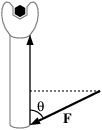
\includegraphics{9_4_Wrench}}
\end{center}
\caption{A wrench.}
\label{F:9.4.Wrench}
\end{minipage}
\end{figure}


\end{pa} \afterpa 